\begin{figure}[htbp]
\section*{ SCO2}
\centering
\begin{subfigure}[b]{0.95\textwidth}
\centering
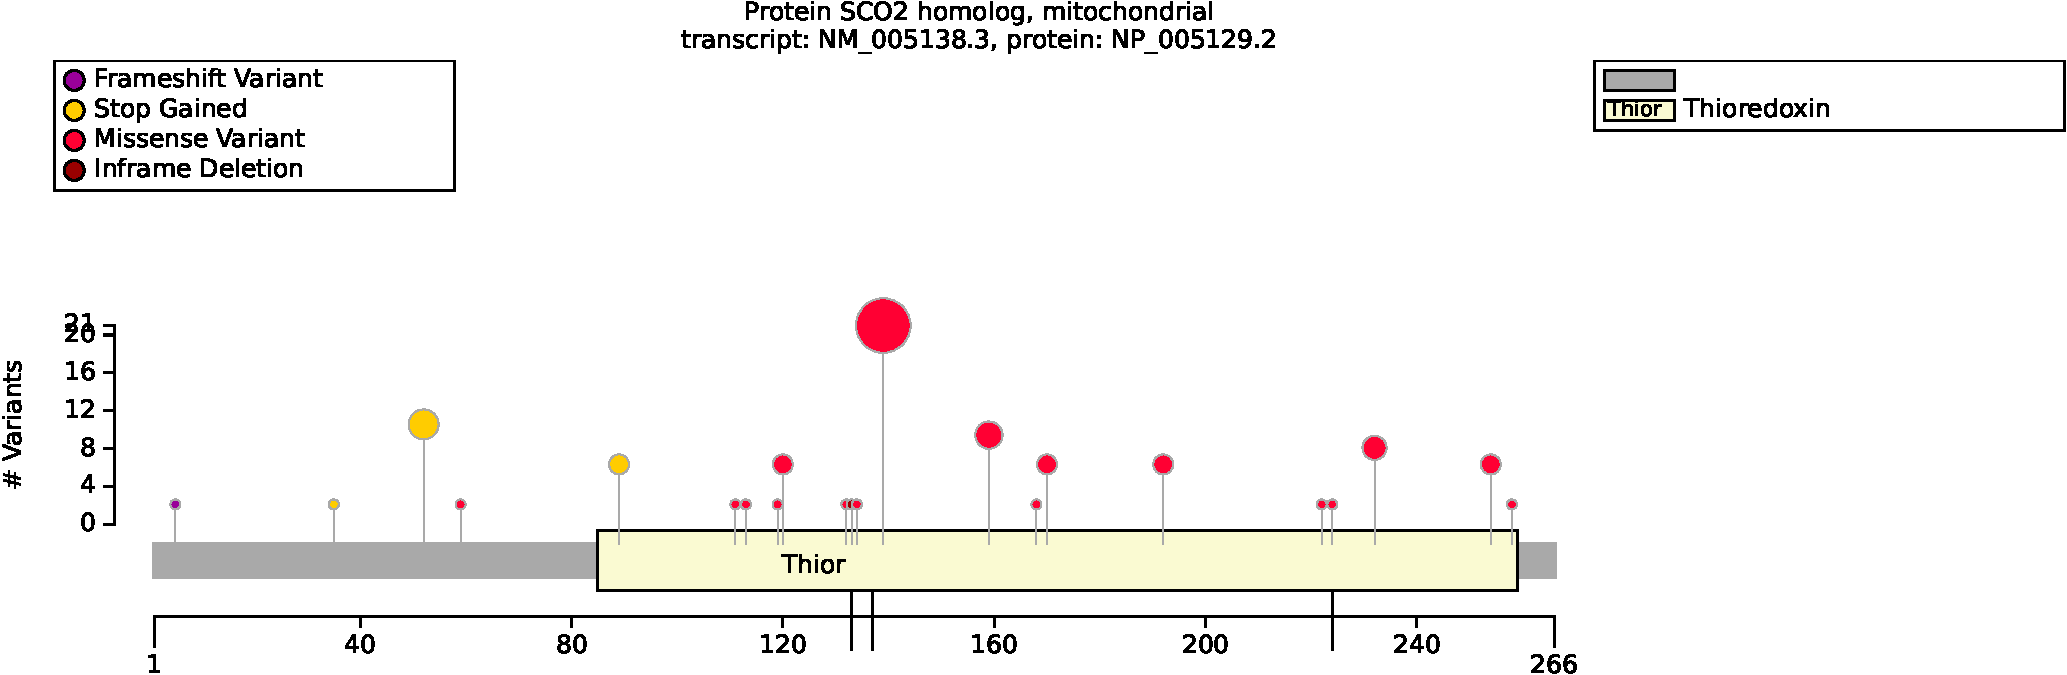
\includegraphics[width=\textwidth]{ img/SCO2_protein_diagram.pdf} 
\captionsetup{justification=raggedright,singlelinecheck=false}
\caption{Distribution of variants in SCO2}
\end{subfigure}

\vspace{2em}

\begin{subfigure}[b]{0.95\textwidth}
\centering
\resizebox{\textwidth}{!}{
\begin{tabular}{llllrr}
\toprule
HPO term & Glu140Lys/Glu140Lys & other/other OR Glu140Lys/other & p-value & adj. p-value\\
\midrule
Hypertrophic cardiomyopathy [HP:0001639] & 2/6 (33\%) & 13/13 (100\%) & 0.004 & 0.027\\
\bottomrule
\end{tabular}
}
\captionsetup{justification=raggedright,singlelinecheck=false}
\caption{Fisher Exact Test performed to compare HPO annotation frequency with respect to Glu140Lys/Glu140Lys and other/other OR Glu140Lys/other. Total of
        7 tests were performed. }
\end{subfigure}
\vspace{2em}
\begin{subfigure}[b]{0.95\textwidth}
\captionsetup{justification=raggedright,singlelinecheck=false}
\resizebox{\textwidth}{!}{
\begin{tabular}{llllrr}
\toprule
Description & Variable & Genotype (A) & Genotype (B) & p-value & xrefs\\
\midrule
Survival analysis: Hypertrophic cardiomyopathy & Onset of HP:0001639 & Glu140Lys/Glu140Lys & other/other OR Glu140Lys/other & 0.219 & -\\
\bottomrule
\end{tabular}
}
\caption{ Onset of Hypertrophic cardiomyopathy to compare Glu140Lys/Glu140Lys and other/other OR Glu140Lys/other with respect to Onset of HP:0001639. }
\end{subfigure}

\vspace{2em}

\begin{subfigure}[b]{0.95\textwidth}
\captionsetup{justification=raggedright,singlelinecheck=false}
\resizebox{\textwidth}{!}{
\begin{tabular}{llllrr}
\toprule
Description & Variable & Genotype (A) & Genotype (B) & p-value & xrefs\\
\midrule
Compute time until OMIM:604377 onset & Onset of OMIM:604377 & Glu140Lys/Glu140Lys & other/other OR Glu140Lys/other & 0.415 & -\\
\bottomrule
\end{tabular}
}
\caption{ Onset of OMIM:604377 to compare Glu140Lys/Glu140Lys and other/other OR Glu140Lys/other with respect to Onset of OMIM:604377. }
\end{subfigure}

\vspace{2em}

\caption{ The cohort comprised 37 individuals (10 females, 23 males, 4 with unknown sex). 24 of these individuals were reported to be deceased. 
A total of 107 HPO terms were used to annotate the cohort. Disease diagnoses: Mitochondrial complex IV deficiency, nuclear type 2 (OMIM:604377) (31 individuals), 
Myopia 6 (OMIM:608908) (6 individuals). The glu140lys correlation is driven by 5 patients found to be homozous for the Glu140Lys variant \cite{PMID_15499950}. 
The children were between the age of 8 months and 1 year and 8 months. Because of the relatively small cohort and the fact that other members of the cohort were not as young, this represents a bias. We therefore investigate the correlation using a survival analysis below. Because the latter was not significant, we regard the following finding to be unsupported and do not report it as a significant finding.  A total of 57 unique variant alleles were found in \textit{SCO2} (transcript: \texttt{NM\_005138.3}, protein id: \texttt{NP\_005129.2}).}
\end{figure}
